
\section{Data Extraction on Longitudinal Data}
The Election Commission of India provides a digitized archive of the results of all elections conducted by it from 1951 in the form of ``statistical reports'' on its website~\cite{StatReportECI}.  Statistical reports for previous years were simply digitized from paper archives. Subsequent reports have been born-digital, but are available as PDF files, with a few recent results in spreadsheet form. Each statistical report contains several sections. The most important and voluminous of these is a section containing detailed constituency-wise election results. This section contains the official record of the election in that constituency and includes the constituency number, names of contesting candidates, the party each represents, and the number of votes polled. It also contains constituency-wide information such as the number of voters and electors, the number of postal ballots, and the number of invalid votes. 

\begin{figure}[h!]
  \centering
  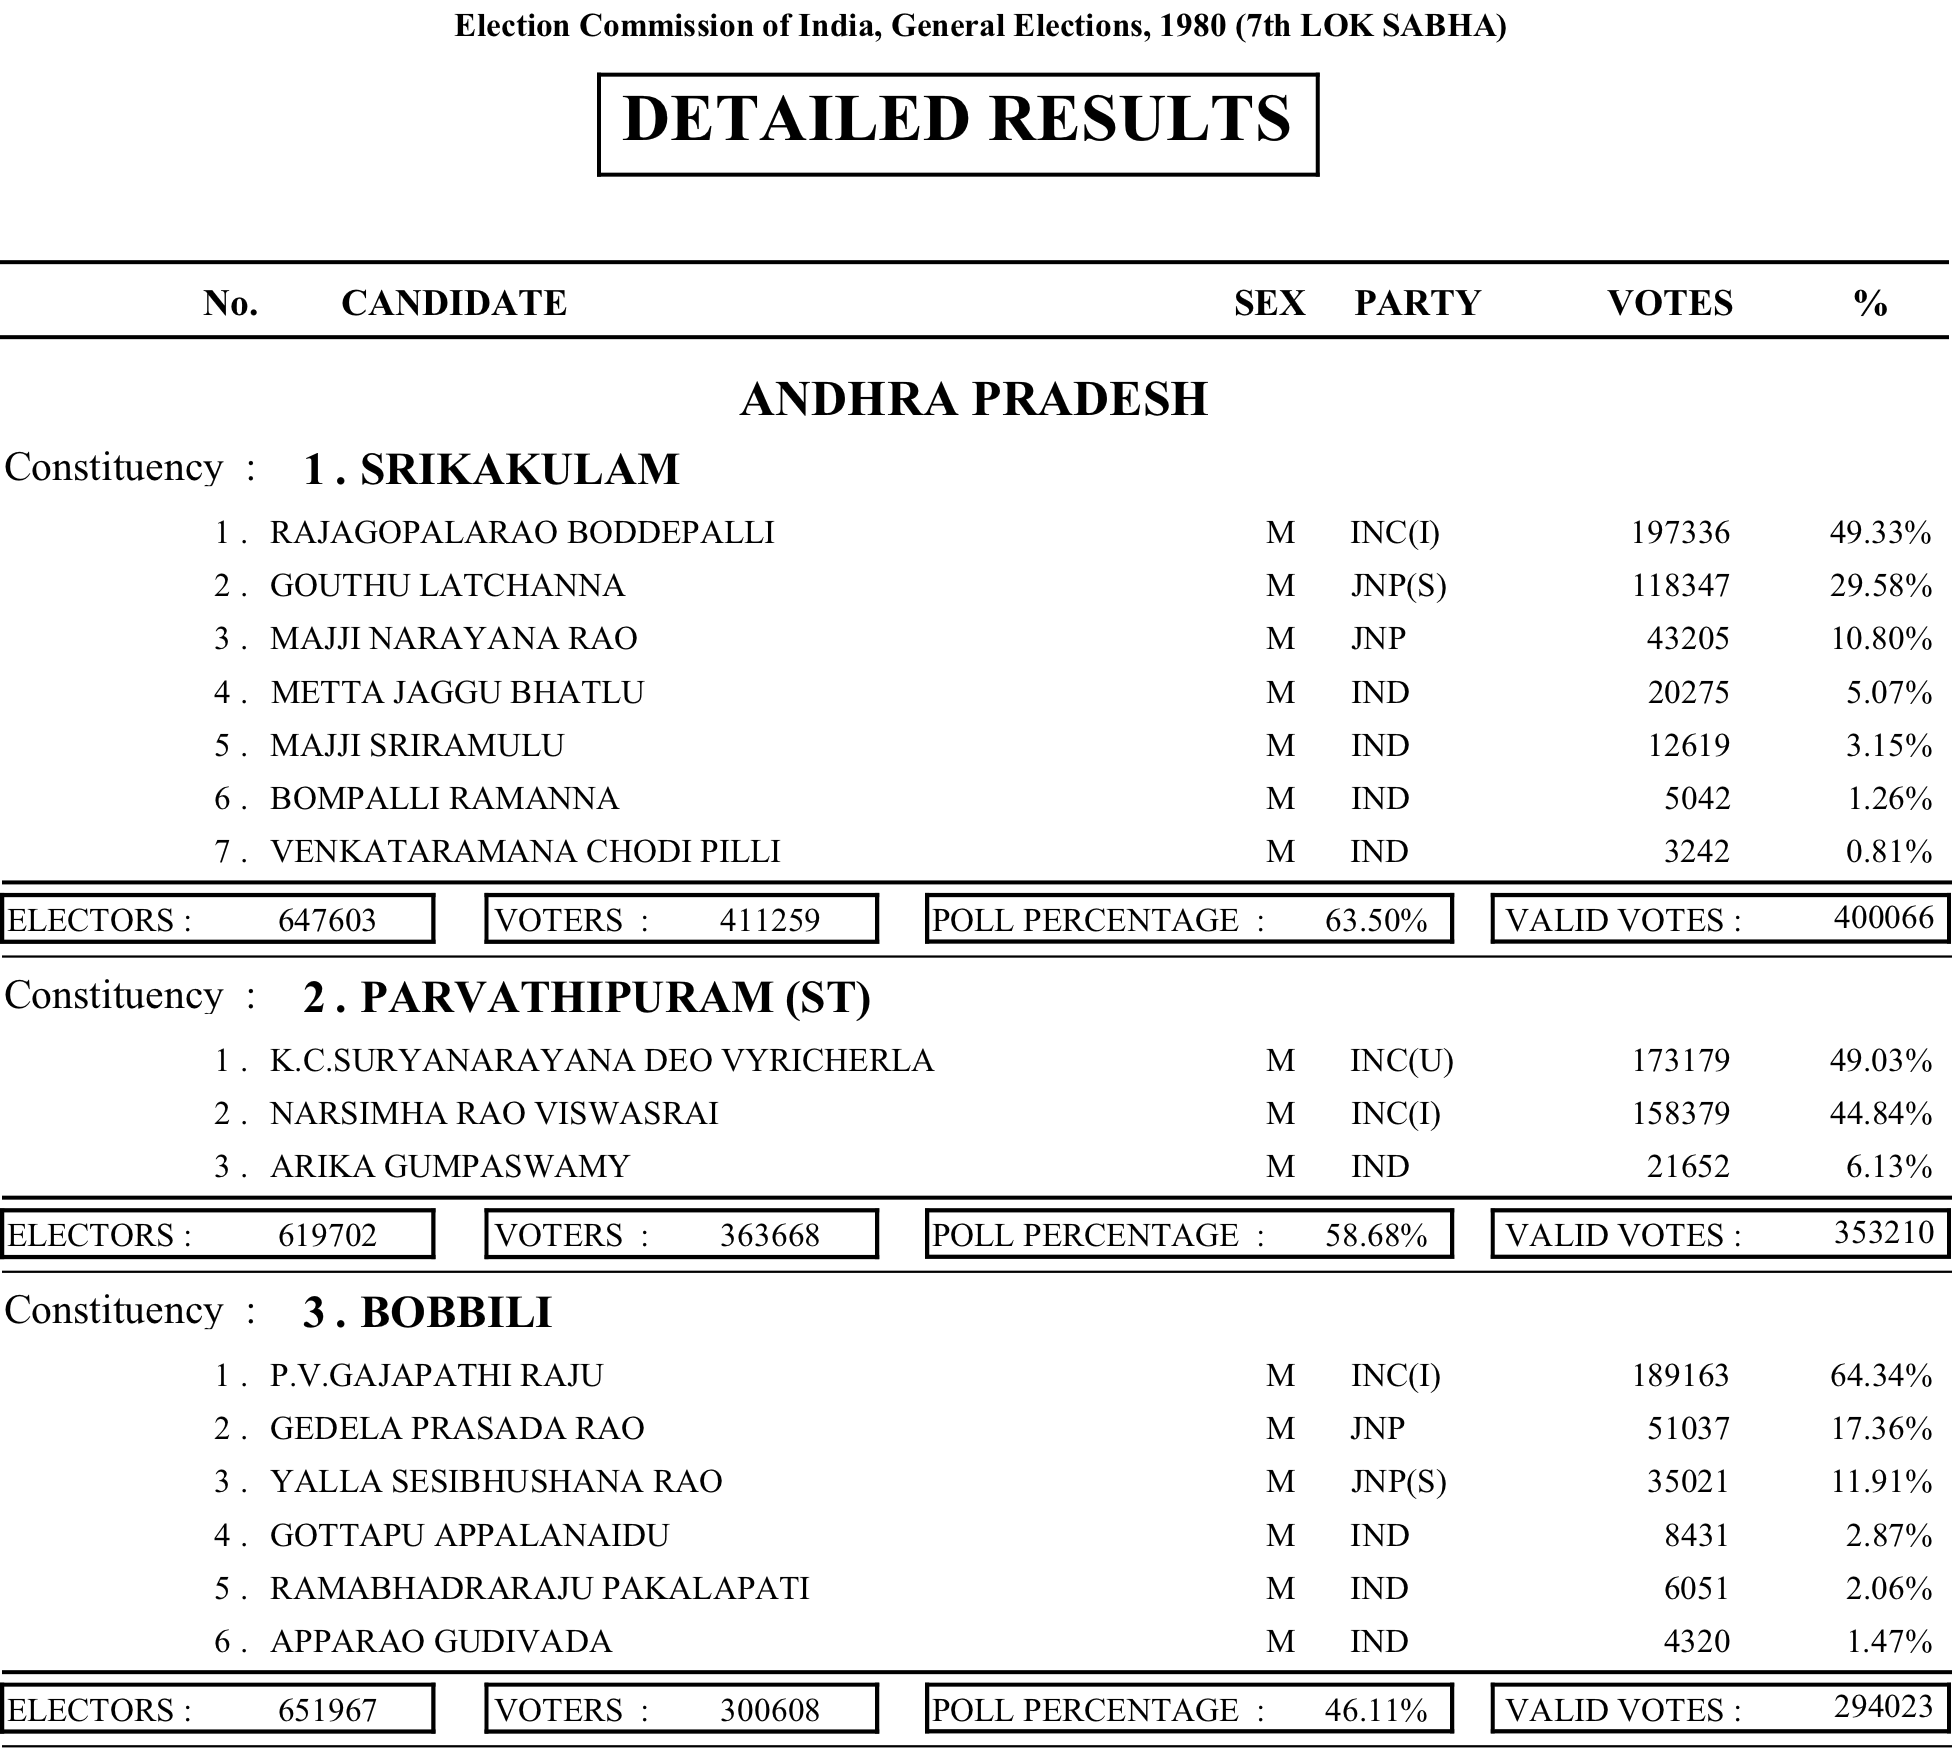
\includegraphics[width=\linewidth]{LS7_DR.png}
  \caption{The Detailed Results section of the statistical report of the 1980 parliamentary elections. The format drifts over time; different reports have different variants of this format.}
%%  \Description{Statistical Report Detailed Results}
  \label{DetailedResults}
\end{figure}


\begin{figure}[h!]
  \centering
  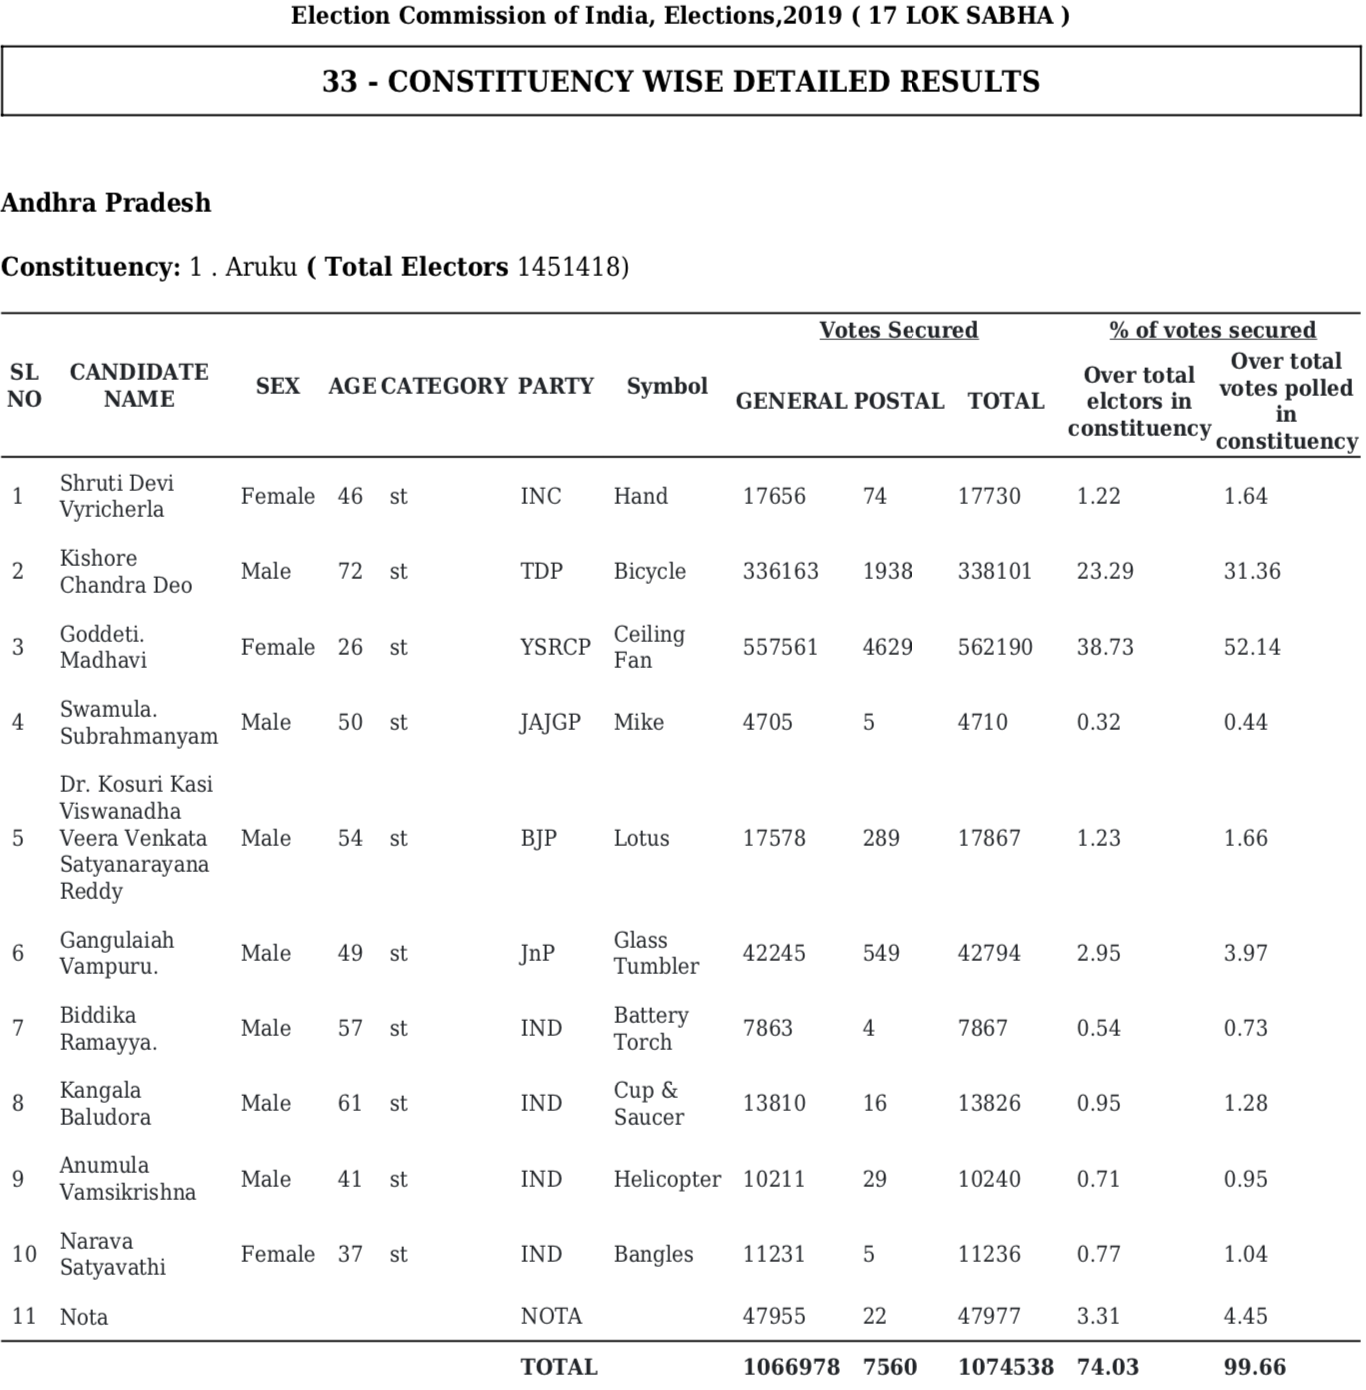
\includegraphics[width=\linewidth]{LS17_DR.png}
  \caption{The Detailed Results section of the statistical report of the 2019 parliamentary elections.}
%%  \Description{Statistical Report Detailed Results}
  \label{DetailedResults17}
\end{figure}
% Some constituencies in India are reserved for Scheduled Castes (SC) and Scheduled Tribes (ST); only candidates from the respective category can contest in them. 

\subsection{Format Drift}

As is often the case with longitudinal data, the formats in these statistical reports have drifted considerably over time. Entire sections have appeared or disappeared in different years; data sections within a page have moved relative to each other, or new fields have got introduced. Figs.~\ref{DetailedResults} and \ref{DetailedResults17}  show the change in format between the 1980 and 2019 statistical reports.

Sections of the source reports often duplicate information, which can lead to inconsistencies. (In database terms, they are non-normalized.) For examples, candidates marked as women in one section of the report may be inconsistently marked as men in another section.

There is also inherent complexity in the data, which needs to be resolved manually. For example, periodic reorganization of Indian states has led to renaming existing states or the creation of new states. These issues can only be tracked manually; LokDhaba handles this by keeping a small set of mapping files to capture this information.

%%The scraped data from general and bye-poll elections is structured as observation variable tables for candidates and constituencies. Each observation for a constituency denotes a contest for a seat in any assembly (state level or parliamentary), and each observation for candidate denotes a candidate who contested any election. The variables capture the information extracted for each observation, which include but not limited to \emph{election type, assembly no, state name, constituency no, poll no, candidate, party, votes}. 
 
\subsection{Data Extraction and Parsing Pipeline}

To design a database for systematically collecting, analyzing and expanding the data on Indian elections, we first needed to extract information about constituencies and candidates from all the statistical reports. The constituency-wise detailed results section contains the electoral information about all the candidates in a given constituency. We build the primary data about candidates by extracting and parsing this section from 342 statistical reports corresponding to all the elections held since 1962. (Elections in prior years had complicated rules like multiple winners in a constituency, making it difficult for our schema to cover them consistently.) 

The structure of this results section varies across the statistical reports in terms of table format and the information present in those tables. Our high-level pipeline to extract, clean and parse this data is shown in Fig. \ref{fig:extraction-pipeline}. This pipeline can be broadly divided into following stages. 
\begin{figure}[h!]
  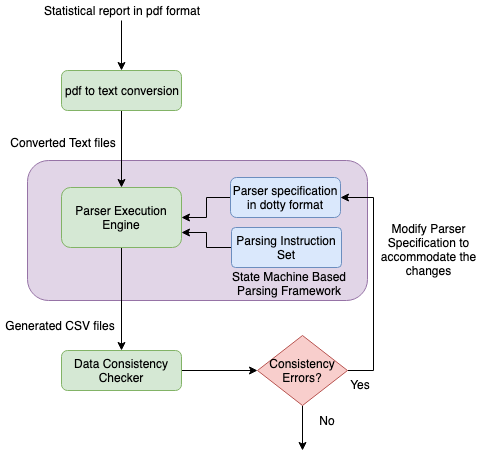
\includegraphics[scale=0.5]{ExtractionPipeline.png}
  \caption{Electoral data extraction pipeline}
  \label{fig:extraction-pipeline}
\end{figure}

\subsubsection{PDF to text conversion} The first step is to use PDF-to-text conversion tools (or optical character recognition tools in some cases) to extract text from the PDF file. If the PDF file was created manually, instead of scanning a paper file, the {\it pdftotext} utility~\cite{pdftotext} gives good results and preserves the layout of the PDF during conversion.

\begin{figure*}
\begin{minipage}{\textwidth}
  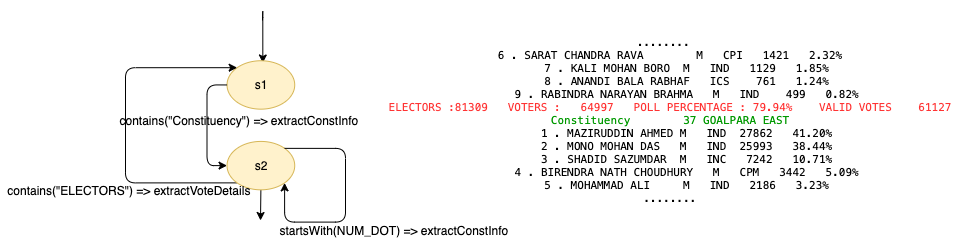
\includegraphics[scale=0.5]{sm-spec.png}
\end{minipage}
\caption{Sample parsing specification program and associated file to parse}
  \label{fig:sample-sm-spec}
\end{figure*}

\subsubsection{Handling format drift} After converting the PDF file to text, we need to parse the text to extract the data in appropriate columns of a structured format. For this purpose, we initially started by developing custom parsers written in the Python programming language. This needed to be done for 342 separate files across all elections. However, the format drift in the tabular structure of these files makes the job of the parser very difficult. Our parser needed a lot of special case handling to handle format mismatches and this was not a solution that would scale and be maintainable in the long run. We have observed that this is a recurrent problem in longitudinal datasets, and therefore it needs a generalizable solution.

Our overall goal is to develop a family of parsers for a set of related formats, in this case, related to Indian elections data. To enable this, we have to come up with a set of parsing rules that are closely tied to the domain and can be easily provided or vetted by domain experts. It is not known how many different parsing specifications will be needed; hence, the specifications themselves need to be iteratively developed as we discover their limitations. In order to detect parsing failures, we need to incorporate a series of consistency checks that pro-actively warn us of such failures, and allow us to develop new specifications or modify existing ones. Consistency checks may be simple (a value in a certain column must be of a certain type) or compound (the values in two columns must satisfy a certain relationship).

Our parsing framework consists of a simple, textually-specified but graphically-viewable programming language. This language captures the essence of the rules needed to parse the family of input files. To develop these specifications, one can write a few simple python functions, and does not need to know any parser generation tools like lex or yacc. The ability to view the parsing specification graphically makes it easy to understand for domain experts who may not be familiar with programming languages.

%\newcommand{trans}{$\delta$}
%\newcommand{lab}{$\sigma$}

A program in our language is represented as a tuple $\left( S,G,A, \mathcal{L} \right)$.  Here $S$ is a set of parsing states, $G$ is a set of guarding conditions, and $A$ is a set of text processing actions. $\mathcal{L}: S \times G \to S \times A$ is a function that assigns a destination state and action to a source state and a guarding condition. Specifically, $\left(s_1,g_1\right) \to \left(s_2,a_1\right) \in \mathcal{L}$ implies a state transition from $s_1$ to $s_2$ if the guarding condition $g_1$ holds at $s_1$; before completing this transition, the text processing action $a_1$ is applied to the input data at $s_1$.  Every guarding condition in $G$ can be of one of the types shown in Table \ref{tab:guarding}. Further, every text parsing action in $A$ can be of one of the types shown in Table \ref{tab:parsingact}. Both the guarding conditions and the parsing actions are fairly domain-specific, but are easy to develop just once, since they refer to intrinsic properties of the data. Hence, their definitions are relatively stable over time.

\begin{figure}[h]
\begin{tabular}{|c|l|} 
 \hline
 \textbf{Condition} & \textbf{Interpretation} \\\hline
 \textbf{true} & always holds true \\\hline
 \textbf{startsWith(s)} & holds true if the line starts with \textbf{s}  \\\hline 
 \textbf{endsWith(s)} & holds true if the line ends with \textbf{s}  \\\hline
 \textbf{contains(s)} & holds true if the line contains string \textbf{s}\\
 \hline
%  \caption{Guarding conditions of the specification language}
%  \label{tab:guarding}
\end{tabular}
\captionof{table}{Guarding conditions\label{tab:guarding}}
\vspace{0.2mm}
\end{figure}

\begin{figure}[h]
\begin{tabular}{|c|l|c|} 
 \hline
 \textbf{Action} & \textbf{Interpretation}& \textbf{\#Variants} \\\hline
 \textbf{extractCandInfo(s)} & \multicolumn{1}{m{3cm}|}{extracts candidate details like name, gender, age, party from string \textbf{s}} &3 \\\hline 
 \textbf{extractConstInfo(s)} & \multicolumn{1}{m{3cm}|}{extracts constitutency details like constituency type, constituency number from  string  \textbf{s}}  & 2 \\\hline
 \textbf{extractVoteDetails(s)} & \multicolumn{1}{m{3cm}|}{extracts vote information from string \textbf{s}} & 1 \\\hline
 \textbf{extractPartyInfo(s)} & \multicolumn{1}{m{3cm}|}{extracts party information like party acronym, full name, party type (national or state) from string \textbf{s}} & 2\\\hline
%  \caption{Text parsing actions of the specification language}
%  \label{tab:parsingact}
\end{tabular}
\captionof{table}{Parsing actions\label{tab:parsingact}}

\end{figure}

The set $A$ consists of parsing functions required to extract useful information from a line of text. For example, the \textbf{extractCandInfo} action specifies that the parser is on the verge of extracting candidate demographic information like name, age, and gender from the upcoming text. The third column of Table \ref{tab:parsingact} represents the number of different variations of each parsing method to cover format drift across different input files. One example of this drift is a rearrangement of the order of fields in candidate information. In some files the candidate's information follows the order of name, age, gender, party, valid votes and total votes. In other files, the order of these fields or the number of fields changed. Due to these issues we created different variants of parsing functions. In all, just 8 parsing actions of four representative methods (\textbf{extractCandInfo}, \textbf{extractConstInfo}, \textbf{extractVoteDetails} and \textbf{extractPartyInfos}) were sufficient to cover all the format drift that we saw in 342 files. 

An example program in our specification language is depicted in Figure \ref{fig:sample-sm-spec}. This program is written to parse candidate information from a text file whose snippet is shown on the right. This snippet, taken from an actual ECI input file, shows the regularity in the structure of the content. It shows a set of lines, one for each candidate's information, followed by a line representing aggregate information (in red), and then followed by the start of information of another constituency. The graphically depicted specification on the left side in Fig. \ref{fig:sample-sm-spec} captures this regularity using two states s1 and s2 and the transitions among them. The transition from s1 to s2 captures the fact that after the aggregate result line in the text snippet (in red) we expect the file to contain a line for the information related to another constituency (in green). The label \textbf{contains("Constituency") => extractConstInfo} on this transition triggers a state change from s1 to s2 if the input line contains the string "Constituency". As a result of this transition, the parsing method \textbf{extractConstInfo} extracts the constituency information from the input line. Further, the fact that there are more than one candidates in a constituency and we need to extract candidate information for all of them is captured by a self transition from s2 to itself. It is to be noted that from a given state more than one transitions can be triggered based on the input data. In this scenario the execution of the parser is stopped with detailed information about the input line in that state. This information is then used to write a more precise specification of the parser so as to traverse only unambiguous transitions.

This specification is passed to a Parser Execution Engine as shown in Fig. \ref{fig:extraction-pipeline}. 
This engine takes a text file as an input and executes the parser specifications to generate a structured database file. Using this approach, we were able to cover the parsing of 342 files by 20 different parser specifications.

\subsubsection{Detecting parsing errors} An important step after getting parsed values from the parsing stage is to perform sanity checks on them. Errors can get introduced at any of the previous stages of the extraction pipeline. For example, PDF to text conversion may not be accurate. Or the parsing phase may wrongly assign the value of one column to another. During our initial development, it was not unusual that a column like, say, `Gender'  would wrongly get mapped into the `Total Votes' column. To detect such anomalies easily and refine our parser, we developed a consistency checking framework. This framework allows domain specialists to express sanity checks for the data in a simple and expressive manner. For example, a person working with electoral data can specify that the number of total votes polled in a constituency should be the sum total of all the votes polled in that constituency by individual candidates. Consistency checks could also be applied to the type of values in a column (a `Gender' column can only contain the values `M', `F', or `O', a `Votes' column can only be a number greater than or equal to 0), or specify constraints between columns. Any violation of such a check indicates a data error has been introduced, and prompts the user to refine the specification or look closely at the source data.

Of course, some of these errors also represent an actual problem in the source data and may require further analysis by a domain expert. Some examples anomalies we observed in our source data were changing of the type of a constituency within a delimitation (which is not expected; see Section \ref{sec:delim}), and more than one candidate from a party contesting in the same constituency.

The consistency checks also helped us to identify special cases in the data that we were unaware of. In constituencies of the Sikkim legislative assembly, we were not aware that the type of a constituency could have the valid tag ``BL'', which marks reservation of the constituency for selected backward classes. We were also able to find out missing results for constituencies. For example, the statistical report for the 7th Parliamentary assembly has data for only 2 constituencies in Assam instead of the expected 10. Similarly, results for \emph{Purnea} constituency in Bihar were missing. Also, comparing total voters to electors in a constituency, as total electors have to be greater than total voters, helped us narrow down errors due to scraping misalignment. The data type checks helped us to identify  missing and incorrect values in bye-elections, missing candidate names in 12 observations, missing votes for a candidate in 56 observations, incorrect constituency or candidate types, and missing gender values in 928 state assembly and 173 national assembly constituencies for 9,104 candidates.

An important objective of our data extraction pipeline is to make the extraction and parsing process as repeatable as possible. This allows us to handle situations when a new version of the data is released, or when better tools become available (say, for OCR) or even when we find a bug in our own tools or processes. Capturing the parsing rules in about 20 high-level directives makes this possible, and is vastly preferable to performing various steps manually.

Our parsing framework can be used in any situation where domain experts and programmers need to work together to convert some source date into a structured format for further processing. It allows non-technical users to effectively take part in the process of data extraction and parsing.
